\section{Umkehrverstärker}
\subsection{Verstärker und Eingangswiderstand}
Zuerst wollen wir die theoretisch zu erwarteten Werte für die Verstärkung und den Eingangswiderstand berechnen:
\begin{align}
    \nu&=\left|-\frac{R_2}{R_1}\right|=\frac{R_2}{R_1}\\
    R_\text{e}&=R_1
\end{align}
Für den Fehler folgt:
\begin{align}
    s_\nu&=\sqrt{\left(\frac{s_{\text{R}_2}}{R_1}\right)^2+\left(\frac{R_2\cdot s_{\text{R}_1}}{R_2^2}\right)^2}\\
    s_{\text{R}_\text{e}}&=s_{\text{R}_1}
\end{align}
Alle Widerstände wurden mit dem Digital-Multimeter nachgemessen.
Ihre Fehler lassen sich folgendermaßen berechnen:
\begin{equation}
    s_\text{R}=\sqrt{s_\text{a}^2+s_\text{r}^2}
\end{equation}
Wobei der Ablesefehler ($s_\text{a}$) und der Restfehler ($s_\text{r}$) dem Protokoll entnommen wurden.\\
Somit ergeben sich folgende Abweichungen bei den verwendeten Widerständen:
\begin{align}
    R_1&=\left(9,99\pm0,10\right)\,\text{k}\Omega\\
    R_2&=\left(1,00\pm0,01\right)\,\text{M}\Omega\\
    R_3&=\left(4,71\pm0,05\right)\,\text{M}\Omega\\
\end{align}
Es folgt für die theoretische Verstärkung:
\begin{framed}
    \begin{align}
        \nu_1^\text{theo}&=100,1\pm1,4& R_\text{e}&=\left(9,99\pm0,10\right)\,\text{k}\Omega &\nu_2^\text{theo}&=471,5\pm6,9
    \end{align}
\end{framed}\newpage
Nun wird die gemessene Verstärkung wie folgt berechnet.
\begin{align}
    \nu&=\frac{U_\text{a}}{U_\text{e}}\\
    s_\nu&=\sqrt{\left(\frac{s_{\text{U}_\text{a}}}{U_\text{e}}\right)^2+\left(\frac{U_\text{a}\cdot s_{\text{U}_\text{e}}}{U_\text{e}^2}\right)^2}\\
    U_\text{a}&=Y\cdot\tilde{U}_\text{Y}\\
    U_\text{e}&=X\cdot\tilde{U}_\text{X}\\
    s_{\text{U}_\text{a}}&=\tilde{U}_\text{Y}\cdot\sqrt{\left(0,5\,\text{div}\right)^2+\left(0,03\cdot Y\right)^2}\\
    s_{\text{U}_\text{e}}&=\tilde{U}_\text{X}\cdot\sqrt{\left(0,5\,\text{div}\right)^2+\left(0,03\cdot X\right)^2}
\end{align}
Für den Fehler wurde ein Ablesefehler von $0,5\,\text{div}$ veranschlagt.
Das Oszilloskop hat eine maximale (interne) Abweichung von $3\%$.
$X$, $Y$ stehen für die abgelesenen 'div' und $\tilde{U}_\text{X}$, $\tilde{U}_\text{Y}$ für die eingestellten '$\frac{\text{V}}{\text{div}}$' des Oszilloskops.
Hierbei steht $X$ für den Kanal 1 (Eingangsspannung) und $Y$ für den Kanal 2 (Ausgangsspannung).\\

Aus den Fragen zur Vorbereitung ist bereits bekannt, dass ein Operationsverstärker keinen unendlich großen Frequenzbereich verstärken kann.
Ab einer gewissen Frequenz nimmt die Verstärkung ab.
Somit wurde der Punkt bei einer Frequenz von $10\,\text{Hz}$ als Referenzwert für die gemessene Verstärkung genommen.
Somit ergeben sich folgende Werte:
\begin{align}
    \nu_1&=\frac{4\,\text{div}\cdot0,5\frac{\text{V}}{\text{div}}}{2\,\text{div}\cdot0,01\frac{\text{V}}{\text{div}}}\\
    \nu_1&=100\\\notag\\
    \nu_2&=\frac{4,5\,\text{div}\cdot2\frac{\text{V}}{\text{div}}}{2\,\text{div}\cdot0,01\frac{\text{V}}{\text{div}}}\\
    \nu_2&=450
\end{align}
Somit ergeben sich folgende experimentell bestimmte Werte:
\begin{framed}
    \begin{align}
        \nu_1^\text{exp}&=100\pm28&\nu_2^\text{exp}&=450\pm125
    \end{align}
\end{framed}
Die experimentell bestimmten Werte, passen mit den theoretisch zu erwarteten Werte hervorragend überein.\newpage
\subsection{Frequenzabhängigkeit der Verstärkung}
Die Verstärkung des Operationsverstärkers wird doppeltlogarithmisch gegen die Kreisfrequenz aufgetragen.
Es ergibt sich folgende Messreihe für die Verstärkung $\nu_1$ ($R_2=1\,\text{M}\Omega$):
\begin{table}[htbp]
    \centering
      \begin{tabular}{c||c|c|c|c}
      $f$ in $\text{Hz}$ & $\omega$ in $\frac{1}{\text{s}}$ & $s_\omega$ in $\frac{1}{\text{s}}$& $\nu$ & $s_\nu$\\
      \hline
      10 & 62,83185307 & 12,56637061 & 100 & 28,27100989\\
      10000 & 62831,8531 & 12,5663706 & 95,0    & 27,1395928 \\
      20000 & 125663,706 & 12,5663706 & 85,0  & 24,9162096 \\
      30000 & 188495,559 & 12,5663706 & 70,0    & 30,660561 \\
      35000 & 219911,486 & 12,5663706 & 70,0    & 30,660561 \\
      40000 & 251327,412 & 12,5663706 & 65,0    & 20,6861669 \\
      50000 & 314159,265 & 12,5663706 & 55,0    & 18,728521 \\
      60000 & 376991,118 & 12,5663706 & 47,5  & 17,3587694 \\
      70000 & 439822,972 & 12,5663706 & 42,5  & 16,5042987 \\
      80000 & 502654,825 & 12,5663706 & 39,0    & 11,0815297 \\
      90000 & 565486,678 & 12,5663706 & 35,0    & 10,1866334 \\
      100000 & 628318,531 & 12,5663706 & 32,0    & 9,53116992 \\
      110000 & 691150,384 & 12,5663706 & 30,0    & 9,10329611 \\
      120000 & 753982,237 & 12,5663706 & 27,0    & 8,47789479 \\
      130000 & 816814,09 & 12,5663706 & 24,0    & 7,87634433 \\
      140000 & 879645,943 & 12,5663706 & 23,0    & 7,68210258 \\
      150000 & 942477,796 & 12,5663706 & 21,0    & 7,30453968 \\
      160000 & 1005309,65 & 12,5663706 & 19,0    & 6,94350776 \\
      170000 & 1068141,5 & 12,5663706 & 15,0    & 4,55164805 \\
      180000 & 1130973,36 & 12,5663706 & 17,0    & 4,98324192 \\
      500000 & 3141592,65 & 12,5663706 & 6,25  & 2,01846941 \\
      1000000 & 6283185,31 & 12,5663706 & 2,5   & 0,80738776 \\
      1500000 & 9424777,96 & 12,5663706 & 1,5   & 0,62823165 \\
      2000000 & 12566370,6 & 12,5663706 & 0,8   & 0,53958503 \\
      \end{tabular}%
      \caption{Messwerte für $\nu_1$ ($R_2=1\,\text{M}\Omega$).}
\end{table}\newpage
Und für $\nu_2$ ($R_2=4,7\,\text{M}\Omega$) folgt:
\begin{table}[htbp]
    \centering
      \begin{tabular}{c||c|c|c|c}
      $f$ in $\text{Hz}$ & $\omega$ in $\frac{1}{\text{s}}$ & $s_\omega$ in $\frac{1}{\text{s}}$ & $\nu$ & $s_\nu$ \\
      \hline
      10 & 62,8318531 & 12,5663706 & 450 & 124,582302 \\
      100 & 628,318531 & 12,5663706 & 470 & 129,243452 \\
      1000 & 6283,18531 & 12,5663706 & 460 & 126,908944 \\
      3000 & 18849,5559 & 12,5663706 & 420 & 117,654239 \\
      4000 & 25132,7412 & 12,5663706 & 400 & 113,08404 \\
      5000 & 31415,9265 & 12,5663706 & 380 & 108,558371 \\
      7000 & 43982,2972 & 12,5663706 & 320 & 95,3116992 \\
      10000 & 62831,8531 & 12,5663706 & 270 & 72,8866929 \\
      11000 & 69115,0384 & 12,5663706 & 250 & 68,1450659 \\
      12000 & 75398,2237 & 12,5663706 & 230 & 63,4544719 \\
      13000 & 81681,409 & 12,5663706 & 220 & 61,1319884 \\
      14000 & 87964,5943 & 12,5663706 & 210 & 58,8271196 \\
      15000 & 94247,7796 & 12,5663706 & 245 & 66,9672121 \\
      16000 & 100530,965 & 12,5663706 & 185 & 53,157008 \\
      17000 & 106814,15 & 12,5663706 & 175 & 50,933167 \\
      18000 & 113097,336 & 12,5663706 & 170 & 49,8324192 \\
      19000 & 119380,521 & 12,5663706 & 160 & 47,6558496 \\
      20000 & 125663,706 & 12,5663706 & 150 & 45,5164805 \\
      25000 & 157079,633 & 12,5663706 & 125 & 40,3693882 \\
      30000 & 188495,559 & 12,5663706 & 105 & 36,5226984 \\
      35000 & 219911,486 & 12,5663706 & 90 & 33,8501108 \\
      40000 & 251327,412 & 12,5663706 & 80 & 32,1950307 \\
      50000 & 314159,265 & 12,5663706 & 63 & 16,7393757 \\
      60000 & 376991,118 & 12,5663706 & 52 & 14,1020282 \\
      80000 & 502654,825 & 12,5663706 & 40 & 11,308404 \\
      200000 & 1256637,06 & 12,5663706 & 16 & 6,43900613 \\
      300000 & 1884955,59 & 12,5663706 & 10 & 3,56089876 \\
      1000000 & 6283185,31 & 12,5663706 & 4 & 2,69792513 \\
      2000000 & 12566370,6 & 12,5663706 & 2,5 & 2,57912291 \\
      \end{tabular}%
      \caption{Messwerte für $\nu_2$ ($R_2=4,7\,\text{M}\Omega$).}
  \end{table}\newpage
Wenn man dies nun in ein Diagramm einzeichnet, ergibt sich folgender Verlauf:
\begin{figure}[h]
    \centering\subfigure[$R_2=1\,\text{M}\Omega$]{\scalebox{1}{% GNUPLOT: LaTeX picture with Postscript
\begingroup
  % Encoding inside the plot.  In the header of your document, this encoding
  % should to defined, e.g., by using
  % \usepackage[cp1252,<other encodings>]{inputenc}
  \inputencoding{cp1252}%
  \makeatletter
  \providecommand\color[2][]{%
    \GenericError{(gnuplot) \space\space\space\@spaces}{%
      Package color not loaded in conjunction with
      terminal option `colourtext'%
    }{See the gnuplot documentation for explanation.%
    }{Either use 'blacktext' in gnuplot or load the package
      color.sty in LaTeX.}%
    \renewcommand\color[2][]{}%
  }%
  \providecommand\includegraphics[2][]{%
    \GenericError{(gnuplot) \space\space\space\@spaces}{%
      Package graphicx or graphics not loaded%
    }{See the gnuplot documentation for explanation.%
    }{The gnuplot epslatex terminal needs graphicx.sty or graphics.sty.}%
    \renewcommand\includegraphics[2][]{}%
  }%
  \providecommand\rotatebox[2]{#2}%
  \@ifundefined{ifGPcolor}{%
    \newif\ifGPcolor
    \GPcolorfalse
  }{}%
  \@ifundefined{ifGPblacktext}{%
    \newif\ifGPblacktext
    \GPblacktexttrue
  }{}%
  % define a \g@addto@macro without @ in the name:
  \let\gplgaddtomacro\g@addto@macro
  % define empty templates for all commands taking text:
  \gdef\gplbacktext{}%
  \gdef\gplfronttext{}%
  \makeatother
  \ifGPblacktext
    % no textcolor at all
    \def\colorrgb#1{}%
    \def\colorgray#1{}%
  \else
    % gray or color?
    \ifGPcolor
      \def\colorrgb#1{\color[rgb]{#1}}%
      \def\colorgray#1{\color[gray]{#1}}%
      \expandafter\def\csname LTw\endcsname{\color{white}}%
      \expandafter\def\csname LTb\endcsname{\color{black}}%
      \expandafter\def\csname LTa\endcsname{\color{black}}%
      \expandafter\def\csname LT0\endcsname{\color[rgb]{1,0,0}}%
      \expandafter\def\csname LT1\endcsname{\color[rgb]{0,1,0}}%
      \expandafter\def\csname LT2\endcsname{\color[rgb]{0,0,1}}%
      \expandafter\def\csname LT3\endcsname{\color[rgb]{1,0,1}}%
      \expandafter\def\csname LT4\endcsname{\color[rgb]{0,1,1}}%
      \expandafter\def\csname LT5\endcsname{\color[rgb]{1,1,0}}%
      \expandafter\def\csname LT6\endcsname{\color[rgb]{0,0,0}}%
      \expandafter\def\csname LT7\endcsname{\color[rgb]{1,0.3,0}}%
      \expandafter\def\csname LT8\endcsname{\color[rgb]{0.5,0.5,0.5}}%
    \else
      % gray
      \def\colorrgb#1{\color{black}}%
      \def\colorgray#1{\color[gray]{#1}}%
      \expandafter\def\csname LTw\endcsname{\color{white}}%
      \expandafter\def\csname LTb\endcsname{\color{black}}%
      \expandafter\def\csname LTa\endcsname{\color{black}}%
      \expandafter\def\csname LT0\endcsname{\color{black}}%
      \expandafter\def\csname LT1\endcsname{\color{black}}%
      \expandafter\def\csname LT2\endcsname{\color{black}}%
      \expandafter\def\csname LT3\endcsname{\color{black}}%
      \expandafter\def\csname LT4\endcsname{\color{black}}%
      \expandafter\def\csname LT5\endcsname{\color{black}}%
      \expandafter\def\csname LT6\endcsname{\color{black}}%
      \expandafter\def\csname LT7\endcsname{\color{black}}%
      \expandafter\def\csname LT8\endcsname{\color{black}}%
    \fi
  \fi
    \setlength{\unitlength}{0.0500bp}%
    \ifx\gptboxheight\undefined%
      \newlength{\gptboxheight}%
      \newlength{\gptboxwidth}%
      \newsavebox{\gptboxtext}%
    \fi%
    \setlength{\fboxrule}{0.5pt}%
    \setlength{\fboxsep}{1pt}%
\begin{picture}(7200.00,5040.00)%
    \gplgaddtomacro\gplbacktext{%
      \csname LTb\endcsname%%
      \put(946,1503){\makebox(0,0)[r]{\strut{}$1$}}%
      \put(946,2557){\makebox(0,0)[r]{\strut{}$10$}}%
      \put(946,3610){\makebox(0,0)[r]{\strut{}$100$}}%
      \put(946,4664){\makebox(0,0)[r]{\strut{}$1000$}}%
      \put(1539,484){\makebox(0,0){\strut{}$100$}}%
      \put(2421,484){\makebox(0,0){\strut{}$1000$}}%
      \put(3303,484){\makebox(0,0){\strut{}$10000$}}%
      \put(4184,484){\makebox(0,0){\strut{}$100000$}}%
      \put(5066,484){\makebox(0,0){\strut{}$1\times10^{6}$}}%
      \put(5948,484){\makebox(0,0){\strut{}$1\times10^{7}$}}%
    }%
    \gplgaddtomacro\gplfronttext{%
      \csname LTb\endcsname%%
      \put(209,2761){\rotatebox{-270}{\makebox(0,0){\strut{}$\nu$}}}%
      \csname LTb\endcsname%%
      \put(6748,2761){\rotatebox{-270}{\makebox(0,0){\strut{}}}}%
      \csname LTb\endcsname%%
      \put(3885,154){\makebox(0,0){\strut{}$\omega$}}%
      \csname LTb\endcsname%%
      \put(3885,4819){\makebox(0,0){\strut{}}}%
      \csname LTb\endcsname%%
      \put(132,-110){\makebox(0,0)[l]{\strut{}}}%
      \csname LTb\endcsname%%
      \put(5706,4646){\makebox(0,0)[r]{\strut{}Messwerte}}%
      \csname LTb\endcsname%%
      \put(3885,33975){\makebox(0,0){\strut{}}}%
    }%
    \gplbacktext
    \put(0,0){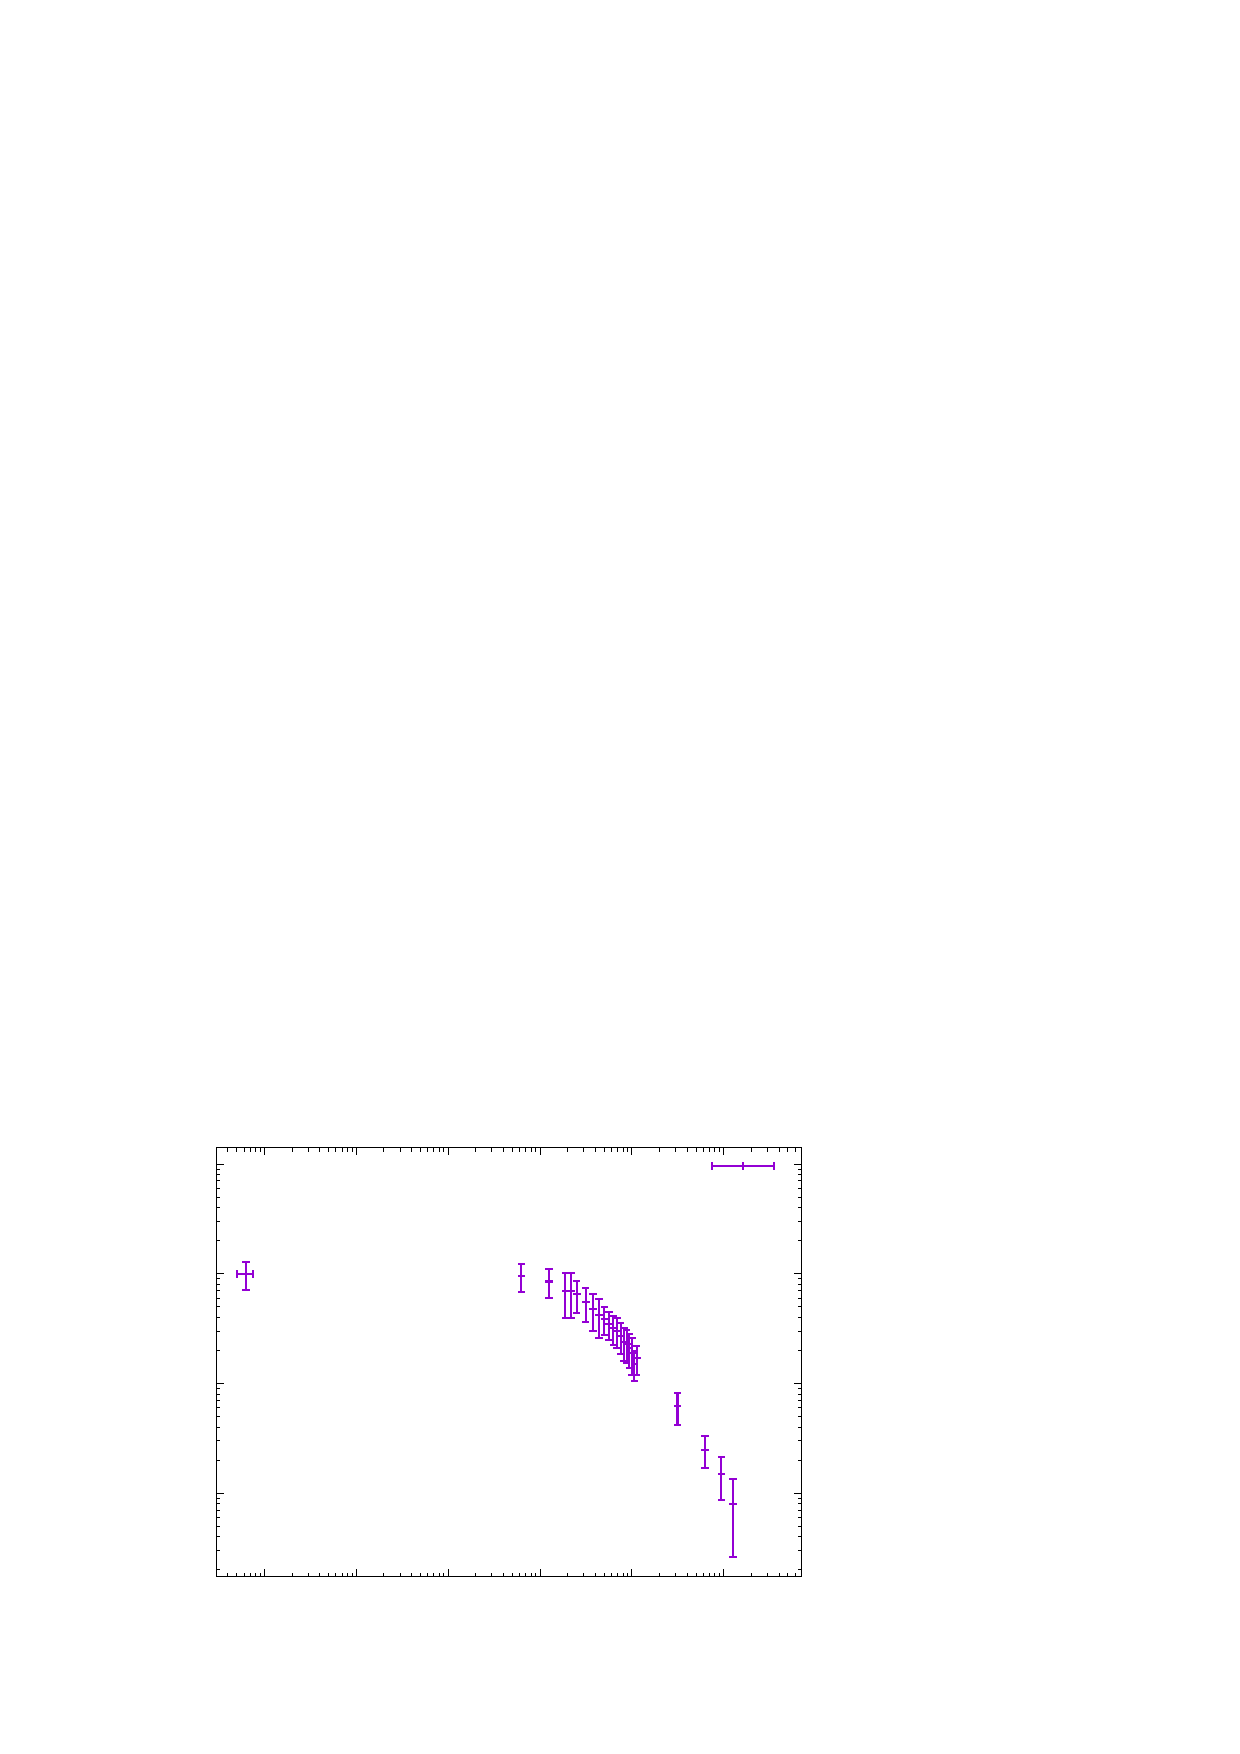
\includegraphics[width={360.00bp},height={252.00bp}]{verstaerkung}}%
    \gplfronttext
  \end{picture}%
\endgroup
}}\\
    \centering\subfigure[$R_2=4,7\,\text{M}\Omega$]{\scalebox{1}{% GNUPLOT: LaTeX picture with Postscript
\begingroup
  % Encoding inside the plot.  In the header of your document, this encoding
  % should to defined, e.g., by using
  % \usepackage[cp1252,<other encodings>]{inputenc}
  \inputencoding{cp1252}%
  \makeatletter
  \providecommand\color[2][]{%
    \GenericError{(gnuplot) \space\space\space\@spaces}{%
      Package color not loaded in conjunction with
      terminal option `colourtext'%
    }{See the gnuplot documentation for explanation.%
    }{Either use 'blacktext' in gnuplot or load the package
      color.sty in LaTeX.}%
    \renewcommand\color[2][]{}%
  }%
  \providecommand\includegraphics[2][]{%
    \GenericError{(gnuplot) \space\space\space\@spaces}{%
      Package graphicx or graphics not loaded%
    }{See the gnuplot documentation for explanation.%
    }{The gnuplot epslatex terminal needs graphicx.sty or graphics.sty.}%
    \renewcommand\includegraphics[2][]{}%
  }%
  \providecommand\rotatebox[2]{#2}%
  \@ifundefined{ifGPcolor}{%
    \newif\ifGPcolor
    \GPcolorfalse
  }{}%
  \@ifundefined{ifGPblacktext}{%
    \newif\ifGPblacktext
    \GPblacktexttrue
  }{}%
  % define a \g@addto@macro without @ in the name:
  \let\gplgaddtomacro\g@addto@macro
  % define empty templates for all commands taking text:
  \gdef\gplbacktext{}%
  \gdef\gplfronttext{}%
  \makeatother
  \ifGPblacktext
    % no textcolor at all
    \def\colorrgb#1{}%
    \def\colorgray#1{}%
  \else
    % gray or color?
    \ifGPcolor
      \def\colorrgb#1{\color[rgb]{#1}}%
      \def\colorgray#1{\color[gray]{#1}}%
      \expandafter\def\csname LTw\endcsname{\color{white}}%
      \expandafter\def\csname LTb\endcsname{\color{black}}%
      \expandafter\def\csname LTa\endcsname{\color{black}}%
      \expandafter\def\csname LT0\endcsname{\color[rgb]{1,0,0}}%
      \expandafter\def\csname LT1\endcsname{\color[rgb]{0,1,0}}%
      \expandafter\def\csname LT2\endcsname{\color[rgb]{0,0,1}}%
      \expandafter\def\csname LT3\endcsname{\color[rgb]{1,0,1}}%
      \expandafter\def\csname LT4\endcsname{\color[rgb]{0,1,1}}%
      \expandafter\def\csname LT5\endcsname{\color[rgb]{1,1,0}}%
      \expandafter\def\csname LT6\endcsname{\color[rgb]{0,0,0}}%
      \expandafter\def\csname LT7\endcsname{\color[rgb]{1,0.3,0}}%
      \expandafter\def\csname LT8\endcsname{\color[rgb]{0.5,0.5,0.5}}%
    \else
      % gray
      \def\colorrgb#1{\color{black}}%
      \def\colorgray#1{\color[gray]{#1}}%
      \expandafter\def\csname LTw\endcsname{\color{white}}%
      \expandafter\def\csname LTb\endcsname{\color{black}}%
      \expandafter\def\csname LTa\endcsname{\color{black}}%
      \expandafter\def\csname LT0\endcsname{\color{black}}%
      \expandafter\def\csname LT1\endcsname{\color{black}}%
      \expandafter\def\csname LT2\endcsname{\color{black}}%
      \expandafter\def\csname LT3\endcsname{\color{black}}%
      \expandafter\def\csname LT4\endcsname{\color{black}}%
      \expandafter\def\csname LT5\endcsname{\color{black}}%
      \expandafter\def\csname LT6\endcsname{\color{black}}%
      \expandafter\def\csname LT7\endcsname{\color{black}}%
      \expandafter\def\csname LT8\endcsname{\color{black}}%
    \fi
  \fi
    \setlength{\unitlength}{0.0500bp}%
    \ifx\gptboxheight\undefined%
      \newlength{\gptboxheight}%
      \newlength{\gptboxwidth}%
      \newsavebox{\gptboxtext}%
    \fi%
    \setlength{\fboxrule}{0.5pt}%
    \setlength{\fboxsep}{1pt}%
\begin{picture}(7200.00,5040.00)%
    \gplgaddtomacro\gplbacktext{%
      \csname LTb\endcsname%%
      \put(946,704){\makebox(0,0)[r]{\strut{}$1$}}%
      \put(946,1951){\makebox(0,0)[r]{\strut{}$10$}}%
      \put(946,3197){\makebox(0,0)[r]{\strut{}$100$}}%
      \put(946,4444){\makebox(0,0)[r]{\strut{}$1000$}}%
      \put(1567,484){\makebox(0,0){\strut{}$100$}}%
      \put(2503,484){\makebox(0,0){\strut{}$1000$}}%
      \put(3439,484){\makebox(0,0){\strut{}$10000$}}%
      \put(4375,484){\makebox(0,0){\strut{}$100000$}}%
      \put(5311,484){\makebox(0,0){\strut{}$1\times10^{6}$}}%
      \put(6246,484){\makebox(0,0){\strut{}$1\times10^{7}$}}%
    }%
    \gplgaddtomacro\gplfronttext{%
      \csname LTb\endcsname%%
      \put(209,2761){\rotatebox{-270}{\makebox(0,0){\strut{}$\nu$}}}%
      \csname LTb\endcsname%%
      \put(6748,2761){\rotatebox{-270}{\makebox(0,0){\strut{}}}}%
      \csname LTb\endcsname%%
      \put(3885,154){\makebox(0,0){\strut{}$\omega$}}%
      \csname LTb\endcsname%%
      \put(3885,4819){\makebox(0,0){\strut{}}}%
      \csname LTb\endcsname%%
      \put(132,-110){\makebox(0,0)[l]{\strut{}}}%
      \csname LTb\endcsname%%
      \put(5706,4646){\makebox(0,0)[r]{\strut{}Messwerte}}%
      \csname LTb\endcsname%%
      \put(3885,274429){\makebox(0,0){\strut{}}}%
    }%
    \gplbacktext
    \put(0,0){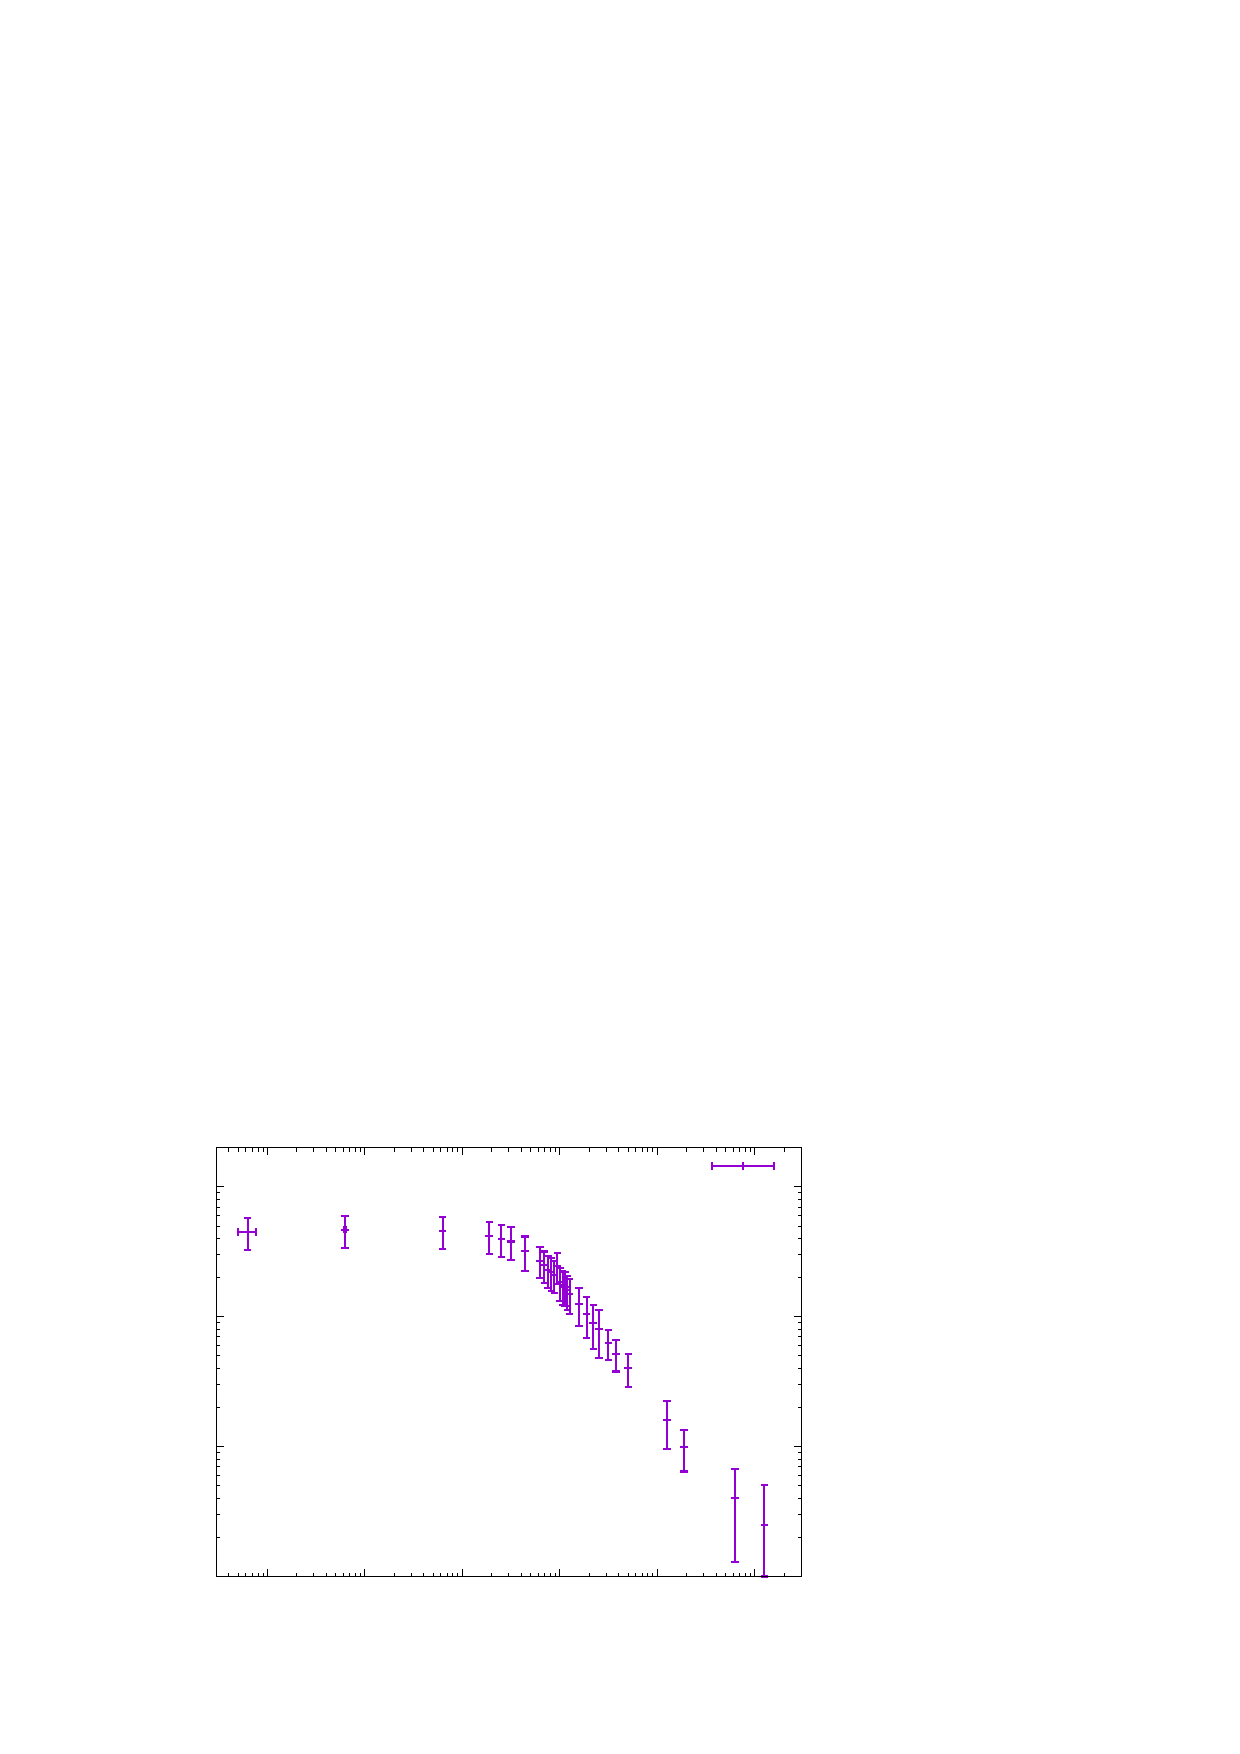
\includegraphics[width={360.00bp},height={252.00bp}]{verstaerkung2}}%
    \gplfronttext
  \end{picture}%
\endgroup
}}
    \caption{Frequenzabhängigkeit der Verstärkung bei verschiedenen Widerständen $R_2$.}
\end{figure}\\
Nun soll das Verstärkung–Bandbreite–Produkt für die beiden Verstärkungen berechnet werden.
Dazu wird der Bereich betrachtet, wo die Verstärkung nicht mehr konstant ist.
Das ist der Frequenzbereich $400-2000\,\text{kHz}$ für $R_2=1\,\text{M}\Omega$ und der Frequenzbereich $7-2000\,\text{kHz}$ für $R_2=4,7\,\text{M}\Omega$.\newpage
Um nun das Verstärkung–Bandbreite–Produkt zu bekommen, wird jede untersuchte Frequenz innerhalb des Frequenzbereiches mit der gemessenen Verstärkung multipliziert und anschließend der Mittelwert gebildet:
\begin{align}
    B\cdot\nu&=\frac{1}{n}\cdot\sum_{i=1}^n\frac{\omega_i}{2\pi}\cdot\nu_i\\
    s_{B\cdot\nu}&=\frac{1}{n}\cdot\sum_{i=1}^n\frac{\sqrt{\left(s_{\omega_i}\cdot\nu_i\right)^2+\left(\omega_i\cdot s_{\nu_i}\right)^2}}{2\pi}\\
\end{align}
Somit folgt für das Verstärkung–Bandbreite–Produkt mit $R_2=1\,\text{M}\Omega$ ($\left(B\cdot\nu\right)^{(1)}$) und mit $R_2=4,7\,\text{M}\Omega$ ($\left(B\cdot\nu\right)^{(2)}$):
\begin{framed}
    \begin{align}
        \left(B\cdot\nu\right)^{(1)}&=f_\text{VBP}^{(1)}=\left(2,8\pm1,0\right)\,\text{MHz} & \left(B\cdot\nu\right)^{(2)}&=f_\text{VBP}^{(2)}=\left(3,1\pm1,2\right)\,\text{MHz}
    \end{align}
\end{framed}
Zu erwarten wäre ein Verstärkung–Bandbreite–Produkt zwischen $2,5\,\text{MHz}$ und $4\,\text{MHz}$ \citep[vgl.][S.6]{tl071}.
Unsere errechneten Werte liegen dazwischen.\newpage
\subsection{Flankenabfallzeit}
Die Bandbreite beschreibt den Frequenzbereich indem die Verstärkung, unabhängig von der eingehenden Frequenz, konstant ist.
Dieser wird durch die Grenzfrequenz abgeschlossen.
Diese Grenzfrequenz kann man mit den Verstärkung–Bandbreite–Produkt berechnen, indem man dieses durch die theoretisch zuerwartente Verstärkung teilt:
\begin{align}
    f_\text{g}&=\frac{f_\text{VBP}}{\nu^\text{theo}}\\
    s_{f_\text{g}}&=\sqrt{\left(\frac{s_{f_\text{VBP}}}{\nu^\text{theo}}\right)^2+\left(\frac{f_\text{VBP}\cdot s_{\nu^\text{theo}}}{\left(\nu^\text{theo}\right)^2}\right)^2}
\end{align}
Somit ergibt sich:
\begin{framed}
    \begin{align}
        f_\text{g}^{(1)}&=\left(28,6\pm9,8\right)\,\text{kHz} & f_\text{g}^{(2)}&=\left(6,7\pm2,5\right)\,\text{kHz}
    \end{align}
\end{framed}
Nun kann man aber auch die Grenzfrequenz mit Hilfe der Flankenabfallzeit, die Zeit, in der das Ausgangssignal auf $\frac{1}{e}$ bei angelegter Rechteckspannung abfällt, bestimmen.
Dazu ist aus dem Versuch komplexe Widerstände bekannt, dass die Beziehung zwischen der Grenzfrequenz, der Bandbreite, und der Flankenabfallzeit umgekehrt proportional ist.
Somit folgt:
\begin{align}
    \frac{1}{\tau}&\overset{!}{=}B=2\pi f_\text{g}\\
    \Leftrightarrow f_\text{g}&=\frac{1}{2\pi\tau}\\
    \tau&=T\cdot\tilde{\tau}\\
    s_{f_\text{g}}&=\frac{s_{\tau}}{2\pi\tau^2}\\
    s_\tau&=\tilde{\tau}\cdot\sqrt{\left(0,2\,\text{div}\right)^2+\left(0,03\cdot T\right)^2}
\end{align}
Für den Fehler wurde wieder ein Ablesefehler von $0,2\,\text{div}$ und ein Restfehler von 3\% veranschlagt.\\
$T$ bezeichnet hier den gemessenen Abstand und $\tilde{\tau}$ die eingestellte Skaleneinteilung.\\
Mit den gemessenen Werten für $\tau$ folgt:
\begin{framed}
    \begin{align}
        f_\text{g}^{(1)}&=\left(19,9\pm5,0\right)\,\text{kHz} & f_\text{g}^{(2)}&=\left(7,2\pm0,4\right)\,\text{kHz}
    \end{align}
\end{framed}
Diese Werte sind geringer, als die Werte welche durch das Verstärkung–Bandbreite–Produkt ausgerechnet wurden.
Aber sie überschneiden sich trotzdem, wenn man die Fehler mitberücksichtigt.
\newpage